\chapter{AdS/CFT correspondence}\label{chp:AdSCFT}


We have seen that a Yang-Mills theory with gauge group $U(N)$ is characterized by two parameters: 
the Yang-Mills coupling $g_\text{YM}$ and the gauge group rank $N$.
Before stating the gauge/string duality, also known as the holographic principle, 
let us discuss different perturbative limits in string theory.

In string theory, there are two parameters used for expansion: 
the string coupling constant $g_s$ and the string length\footnote{
It is a fundamental scale in string theory, and not literally the length of the strings.} $l_s = \sqrt{\alpha'}$.
% where $\alpha'$ is called the Regge slope, 
% and it is related to the string tension $T_\text{F1}=1/(2\pi\alpha')$.
When the string coupling is small, it leads to classical strings,
where only tree level diagrams are taken into account.
This means strings do not merge and split, 
which would give different worldsheet topologies, see figure \ref{fig:stringPerturbation}.
If the strings propagate in a curved background with a characteristic length scale $L$,
the classical gravity limit is obtained by requiring additionally $l_s \ll L$.
In other words, strings can be approximated by point particles (their center mass). 

\begin{figure}[t]
\begin{center}
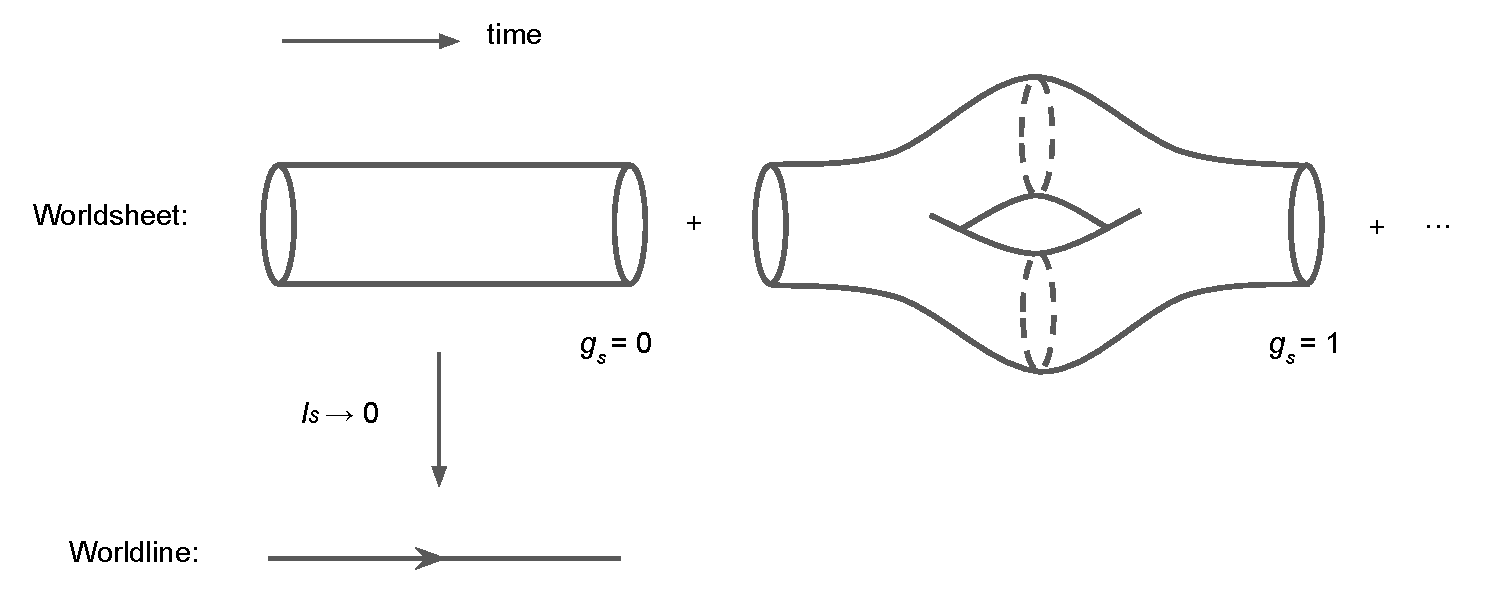
\includegraphics[width=\textwidth]{Images/stringPerturbation.pdf}
\end{center}
\caption{\label{fig:stringPerturbation} Genus expansion of the closed string worldsheet and the point-particle approximation.}
\end{figure}


The AdS/CFT correspondence was originally conjectured by Maldacena \cite{Maldacena:1997re}, 
and stated the below theories are dynamically equivalent:
\begin{itemize}
 \item $\mathcal{N}= 4$ SYM in 4 dimensions with gauge group $SU(N)$
 \item Type IIB superstring theory on $AdS_5 \times S^5$ (both with the same radius L), 
       where the $F_{(5)}$ has integer flux $N$ on $S^5$.
\end{itemize}
The parameters of these two theories are related as:
\begin{equation}\label{couplings}
 g_\text{YM}^2 = 4 \pi g_s, \quad  \lambda \equiv g_\text{YM}^2 N = \left(\dfrac{L}{l_s}\right)^4.
\end{equation}

The conjecture was further developed by \cite{Gubser:1998bc, Witten:1998qj},
and since its original inception, other examples have been found such as
a lower dimensional correspondence between a 3d CFT called ABJM theory 
and type IIA superstring on $AdS_4 \times CP^3$ \cite{Aharony:2008ug}, known as $AdS_4/CFT_3$ correspondence.
It is also an active field of research, but here, we will focus only on the $\mathcal{N}= 4$ case.



We see the first relation in \eqref{couplings} implies the YM's coupling to be small in the classical strings limit.
Moreover, from the second relation, $L/l_s $ is arbitrary in this limit, 
hence $N$ must be large to compensate the smallness of $g_\text{YM}$.
The 't Hooft coupling $\lambda $ is then kept fixed when $N$ is large.
This limit gives planar Feynman diagrams, see figure \ref{fig:planarNonPlanar}, in the leading order on the gauge theory side, 
and corresponds to the genus expansion in string worldsheet, see figure \ref{fig:stringPerturbation}.
This was actually noticed by 't Hooft long before the advent of AdS/CFT correspondence \cite{tHooft:1973alw},
and suggested planar diagrams as triangulations of the string worldsheet.
Notice that, in the planar limit, the Lie groups $U(N)$ and $SU(N)$ are indistinguishable.
% the same, and differ at higher orders in $1/N^2$. 
% It is actually not completely clear which one of these is the gauge group in the correspondence.

\begin{figure}[t]
\begin{center}
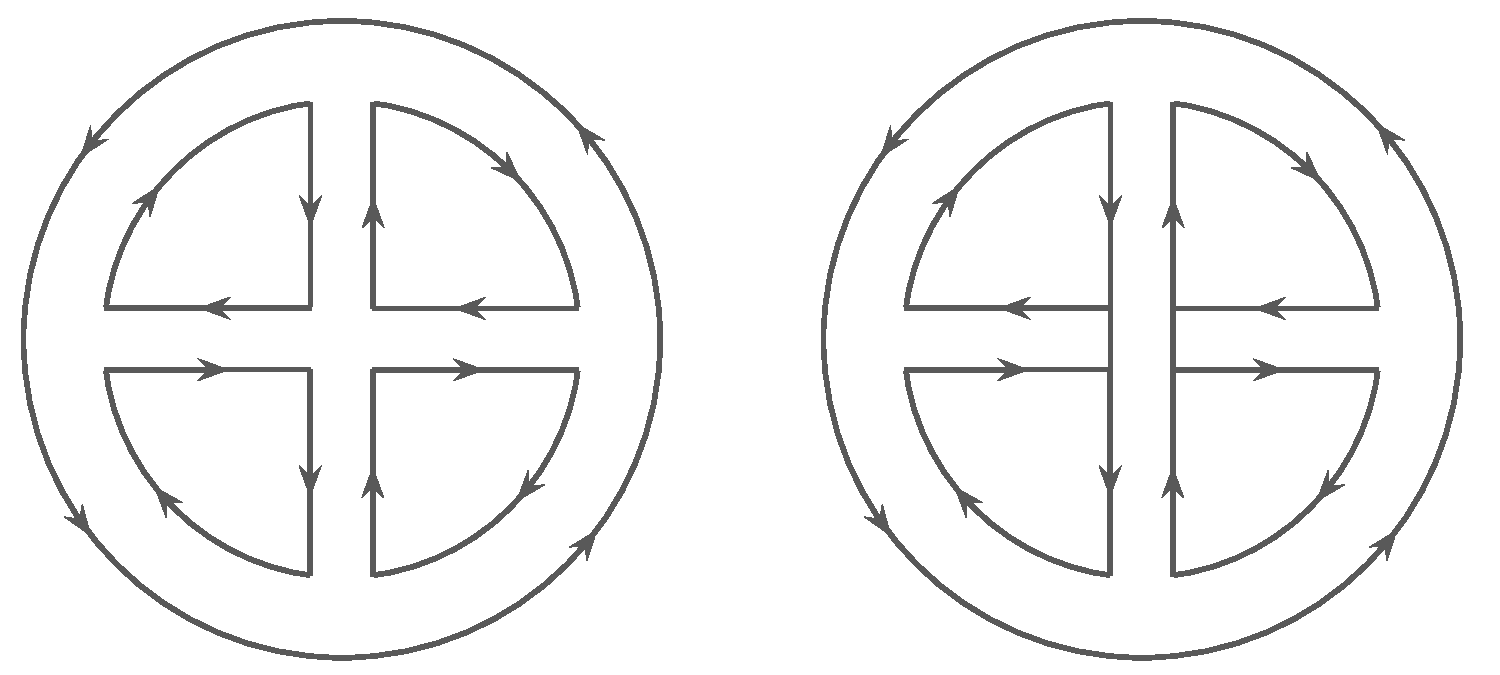
\includegraphics[width=0.7\textwidth]{Images/planarNonPlanar.pdf}
\end{center}
\caption{\label{fig:planarNonPlanar} A planar diagram (left) and a non-planar diagram (right).}
\end{figure}


If we further impose classical gravity limit, then
the 't Hooft coupling must be large too. 
Hence, the correspondence becomes a form of strong/weak duality.
This is the 't Hooft limit and it is the most computationally accessible one, 
since our understanding of string theory beyond the above-mentioned perturbative regimes is poor. 
Moreover, it is potentially seen as a tool to solve strongly coupled quantum field theory using supergravity.
Let us summarize the different limits in the table below:
\begin{center}
 \begin{tabular}{| l | l |}
 \hline
  $\mathcal{N}=4$ SYM & Type IIB strings on $AdS_5 \times S^5$ \\ \hline
  $N, \quad \lambda = g_{YM}^2 N$            & $g_s = \frac{\lambda}{4\pi N}, \quad T = \frac{\sqrt{\lambda}}{2 \pi} $ \\ %(quantum superstring) \\
  $N\rightarrow \infty, \quad \lambda$ fixed & $g_s=0, \quad T$ fixed \\  %(classical superstring) 
  $N\rightarrow \infty, \quad \lambda \rightarrow \infty$ & $g_s=0, \quad T \rightarrow \infty$ \\\hline %   (classical supergravity )
%    Local operators & String states  \\
\end{tabular}
\end{center}

Symmetry-wise, the conjecture is consistent:
\begin{center}
 \begin{tabular}{| l | l |}
 \hline
  $\mathcal{N}=4$ SYM    & Type IIB strings on $AdS_5 \times S^5$ \\ \hline
   conformal symmetry $SO(4,2)$   & isometry of $AdS_5$: $SO(4,2)$ \\ 
   R-symmetry $SO(6)$             & isometry of $S^5$: $SO(6)$ \\ 
   SUSY: 32 supercharges          & SUSY: 32 supercharges \\ \hline
%    Local operators & String states  \\
\end{tabular}
\end{center}

As for local operators in CFT, the AdS/CFT statement is that\footnote{It is generalized to asymptotic $AdS$ spaces, such as the Pilch-Warner geometry.}
\begin{equation}
 \int_{\phi\sim\phi_{(0)}} D\phi e^{-S_\text{string}[\phi]} = \braket{e^{-\int_{\partial AdS} \phi_{(0)} O }}_{CFT},
\end{equation}
where $\phi_{(0)}$ represents the boundary values of fields $\phi$ living in the bulk of $AdS$.
In the supergravity limit, the on-shell supergravity action corresponds to the generating function of connected graphs in the field theory.
In other words, bulk fields with non-trivial boundary values are sources of gauge invariant operators in CFT.
Since the volume of $AdS$ is infinite (due to the second order pole in the radial coordinate),
the divergences are removed using \emph{holographic renormalization}, 
which is analogous to the renormalization of correlation functions.
Holographic renormalization consists of expanding bulk fields close to the boundary, 
identifying the divergent terms and remove them by counterterms, as in the usual renormalization procedure, see e.g. \cite{Skenderis:2002wp} for a review.
% This is also the procedure used to find the holographic dual of N=2*, 
% by solving the non the asymptotic AdS spaces such as Pilch-Warner geometry. 

A formal proof of AdS/CFT correspondence is yet elusive, despite numerous explicit checks.
Next, we will review the original argument from \cite{Maldacena:1997re}.

% \section{Holographic re}


\section{N D3-branes}

The origin of this correspondence lies on the two perspectives of D-branes in superstring theory.

D-branes are non-perturbative objects where open strings end (with Dirichlet conditions, i.e. fixed endpoint with zero momentum). 
In the weak coupling limit $g_s \ll 1$, 
open strings can be thought as excitations of D-branes, see e.g. figure \ref{fig:2Dbranes}.
In the low energy limit $E \ll 1/l_s$, the massive string excitations can be ignored.

Consider a single D3-brane and let us expand its action (the DBI part) for $l_s \ll 1$, 
which gives the low energy open (bosonic) string action:
\begin{equation}
 S = - \dfrac{1}{2 \pi g_s} \int d^{4}x \, (1+\dfrac{1}{4} F^{\mu \nu} F_{\mu \nu} 
     + \dfrac{1}{2} \partial_\mu \Phi_I \partial^{\mu} \Phi^I +\ldots). %+ \mathcal{O}(\alpha'))
\end{equation}
These fields are the gauge field $F_{\mu \nu}$ that transforms in the unbroken Lorentz symmetry of the 4-dimensional worldvolume,
% indexed by $\mu, \nu = 1,2,3$,
and massless scalar fields $\Phi^I$  that are Goldstone bosons of the broken translation symmetry in the six transverse directions of the target space,
due to the presence of the brane. 
The resulting effective theory (excluding the term with no fields) is a $U(1)$ gauge theory living in the worldvolume of the D3-brane.
This identifies the string coupling constant with the Yang-Mills coupling: $4 \pi g_s = g_\text{YM}^2$.
The gauge group is $U(1)$ for a single D-brane, and for $N$ D-branes, 
it gets enhanced from $U(1)^N$ to $U(N)$ if they are coincident, see explanations in \cite{Wulff:2007vj}.
The effective coupling constant is then given by $g_s N$.
% Therefore, this perspective is only reliable for $g_s N \ll 1$.
The full spectrum also contains closed string modes and interaction terms, 
but by carefully taking the low energy limit, these sectors decouple and the interaction term vanishes.

\begin{figure}[t]
\begin{center}
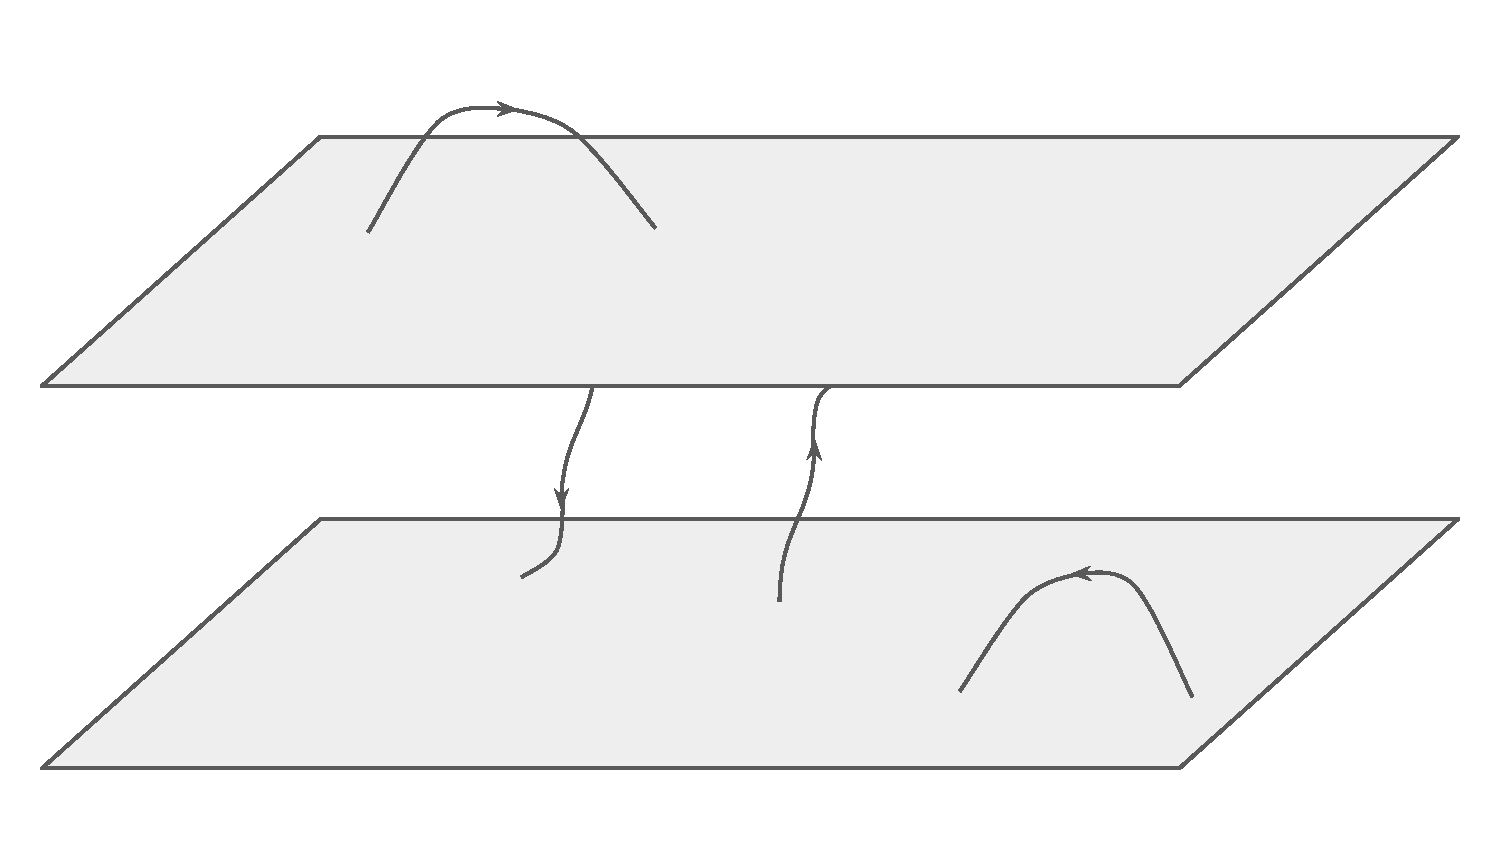
\includegraphics[width=0.6\textwidth]{Images/2Dbranes.pdf}
\end{center}
\caption{\label{fig:2Dbranes} All the possible (oriented) open string excitations in two D-branes. 
If we have $N$ non-coincident D-branes, then there are $N^2$ possible open string configurations.}
\end{figure}

% If we have N non-coincident D-branes, then there are $N^2$ possible open string configurations characterized by their endpoints
% (e.g. for $$\mathcal{N}=2$$, we have (1,1), (1,2), (2,1), (2,2), where the tuple represents the two branes).
% These can be encoded in a $N\times N$ matrix. 

On the other hand, D-branes are also solutions of supergravity field equations, as discussed in chapter \ref{ch:supergravity}.
Hence, as gravitational objects, they can deform the surrounding spacetime, and closed strings can propagate there.
% The supergravity limit is a low energy limit of superstring theory. 
For a stack of $N$ coincident D3-branes, the metric is
\begin{equation}
 ds^2 = \left( 1 + \dfrac{L^4}{r^4} \right)^{-1/2} \eta_{i j} dx^i dx^j  + \left( 1 + \dfrac{L^4}{r^4} \right)^{1/2} (dr^2 + r^2 d\Omega_5^2).
\end{equation}
Notice the two limits for this metric:
\begin{itemize}
 \item $r \gg L$: leading to the 10-dimensional flat Minkowski metric.
 \item $r \ll L$: redefining $z\equiv L^2 / r$, we get the Poincar\'e patch for $AdS_5 \times S^5$. 
\end{itemize} 
% Inserting the full metric to the bosonic string action (non-linear sigma model), we get 
The characteristic length scale \eqref{characteristicLengthLp} in this case is
\begin{equation}
 \dfrac{L^4}{l_s^4} = 4 \pi g_s N.
\end{equation}
By taking the low energy (Maldacena) limit: $l_s \rightarrow 0$ while $L/l_s$ fixed, we can decouple the two sectors,
where the flat space part gets canceled exactly with the closed string modes in the open string analysis.
We arrive now the conclusion of the AdS/CFT correspondence.
However, instead of $U(N)$, we have $SU(N)$, because there is an overall $U(1)$ phase that decouples,
and this degree of freedom corresponds to a boundary field that cannot propagate into the bulk of $AdS_5$.



